%!TEX root = report.tex
This section presents the results of the experiments introduced in \cref{sub:method:design}. In \cref{sub:results:experimental} we show the results of our experiments, \cref{sub:results:interpretation} interprets the found data.

\subsection{Experimental Findings}
\label{sub:results:experimental}
\Cref{fig:results:merging} presents the results of our experiments with the graph where cars had to zip merge. \Cref{fig:results:intersecting} shows the mean average speed for different routes in the graph where cars have to cross an intersection. We distinguish two different groups of routes within this graph, namely straight routes and routes that contain a bend. 

\begin{figure}
	\centering
	\begin{subfigure}{\textwidth}
		\centering
		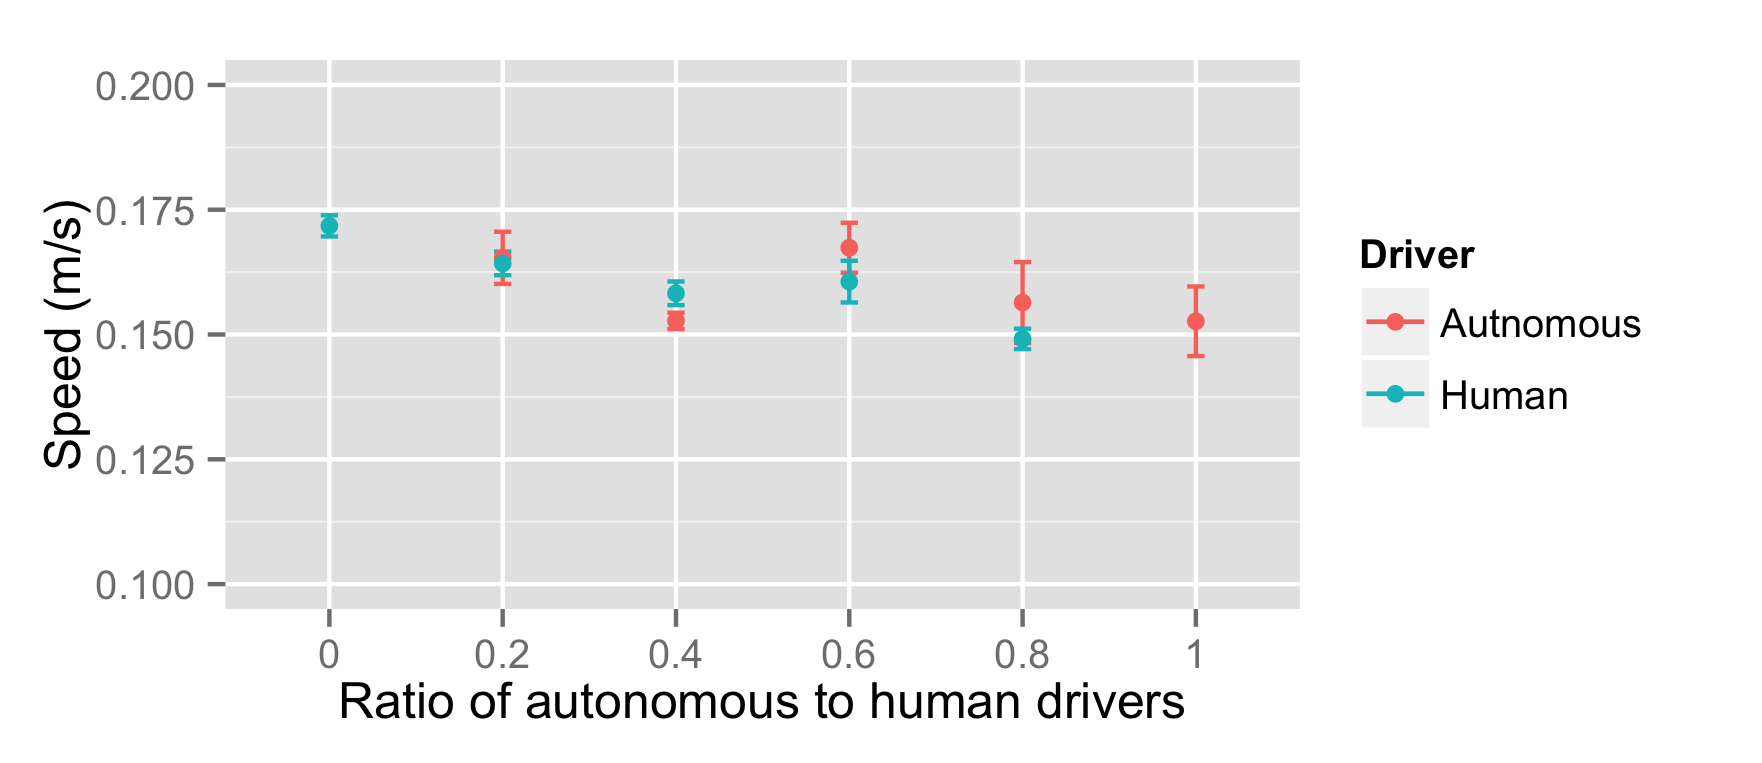
\includegraphics[width=\textwidth]{./img/merging_03}
		\caption{The route from node $S_0$ to node $S_2$.}
		\label{fig:results:merging:03}
	\end{subfigure}
	\begin{subfigure}{\textwidth}
		\centering
		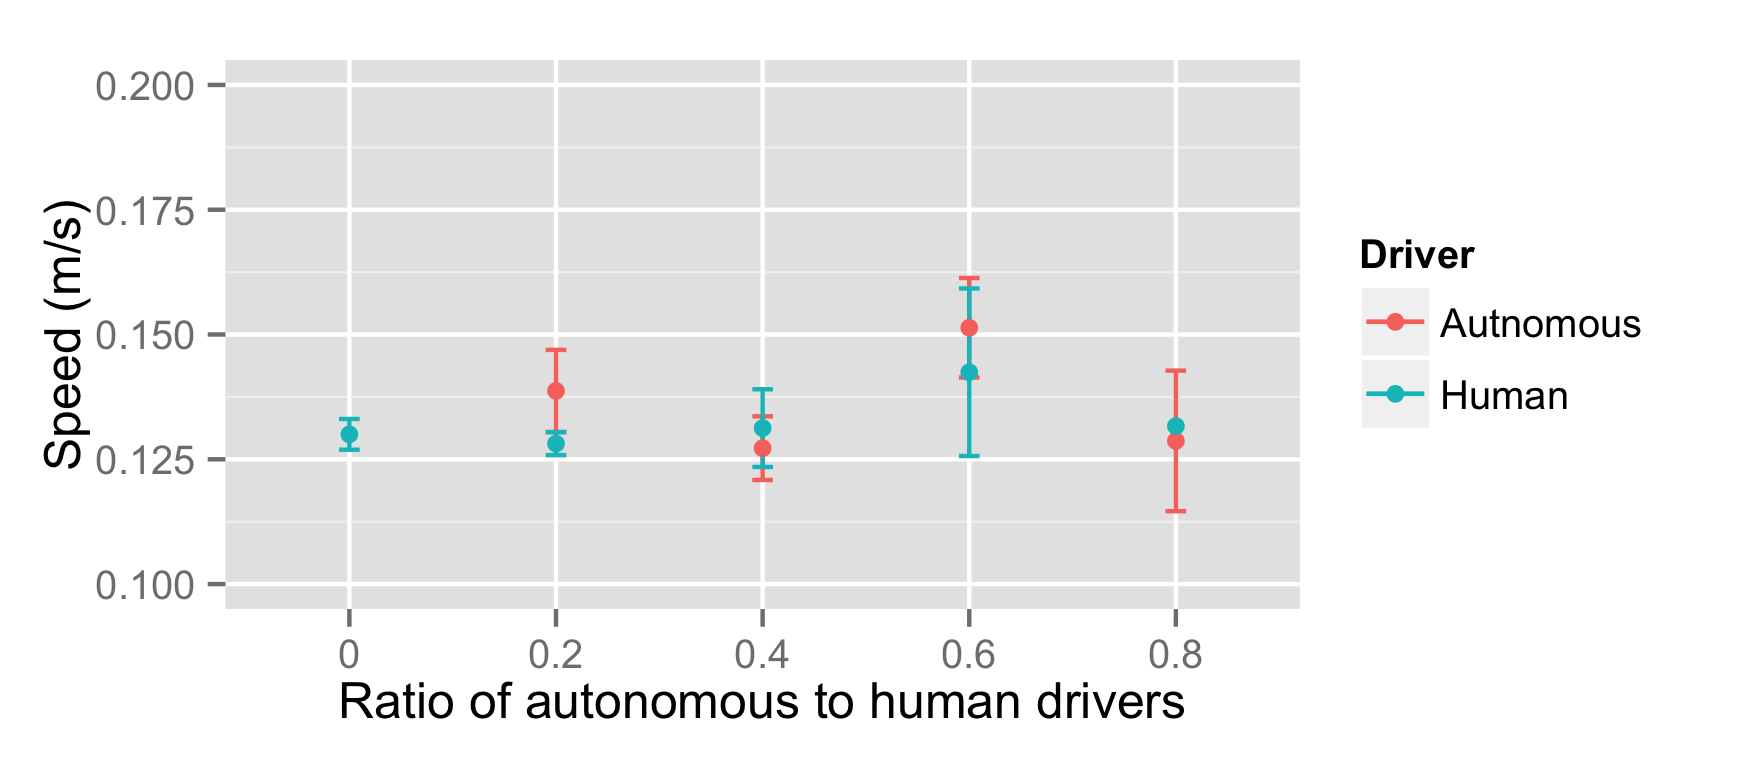
\includegraphics[width=\textwidth]{./img/merging_13}
		\caption{The route from node $S_1$ to node $S_2$.}
		\label{fig:results:merging:13}
	\end{subfigure}	
	\begin{subfigure}{\textwidth}
		\centering
		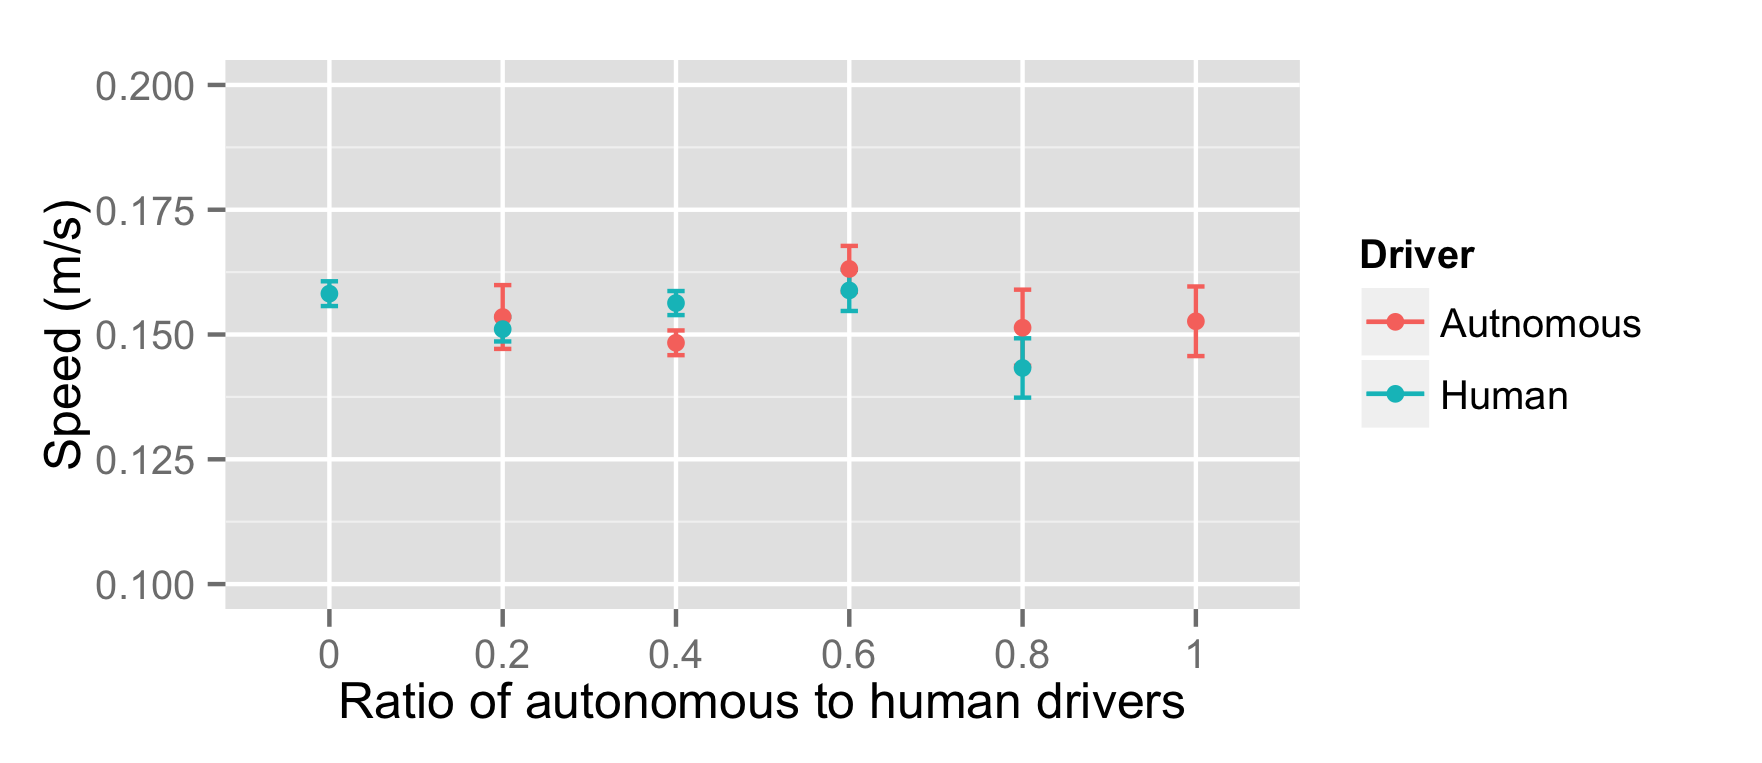
\includegraphics[width=\textwidth]{./img/merging}
		\caption{The route of all routes.}
		\label{fig:results:merging:all}
	\end{subfigure}		
	\caption{Results of the `merging' graph presented in \cref{fig:method:experiment:merging}. Each figure presents the mean average speed over different iterations as a function of the autonomous to human ratio for a different set of routes. \ref{fig:results:merging:03} shows the mean average speed for the route from node $S_0$ to $S_2$, \ref{fig:results:merging:13} for the route from node $S_1$ to $S_2$, and \ref{fig:results:merging:all} shows the mean average speed for all routes.}
	\label{fig:results:merging}
\end{figure}

\begin{figure}
	\centering
	\begin{subfigure}{\textwidth}
		\centering
		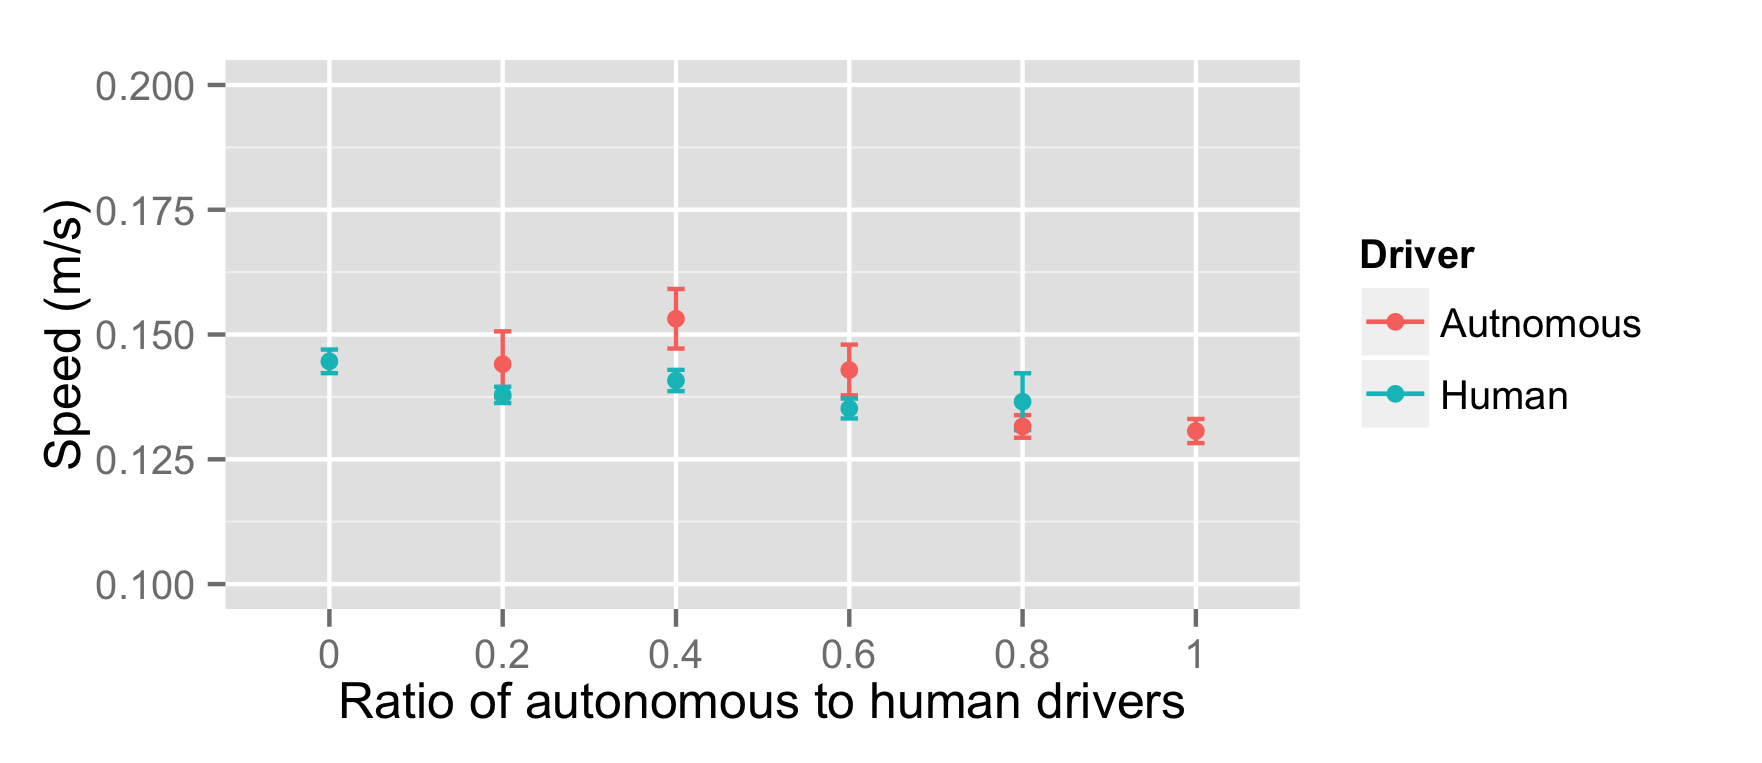
\includegraphics[width=\textwidth]{./img/intersecting_03_01}
		\caption{The routes from node $S_0$ to node $S_3$, $S_0$ to node $S_2$, $S_2$ to node $S_0$ and $S_3$ to node $S_0$.}
		\label{fig:results:intersecting:03}
	\end{subfigure}
	\begin{subfigure}{\textwidth}
		\centering
		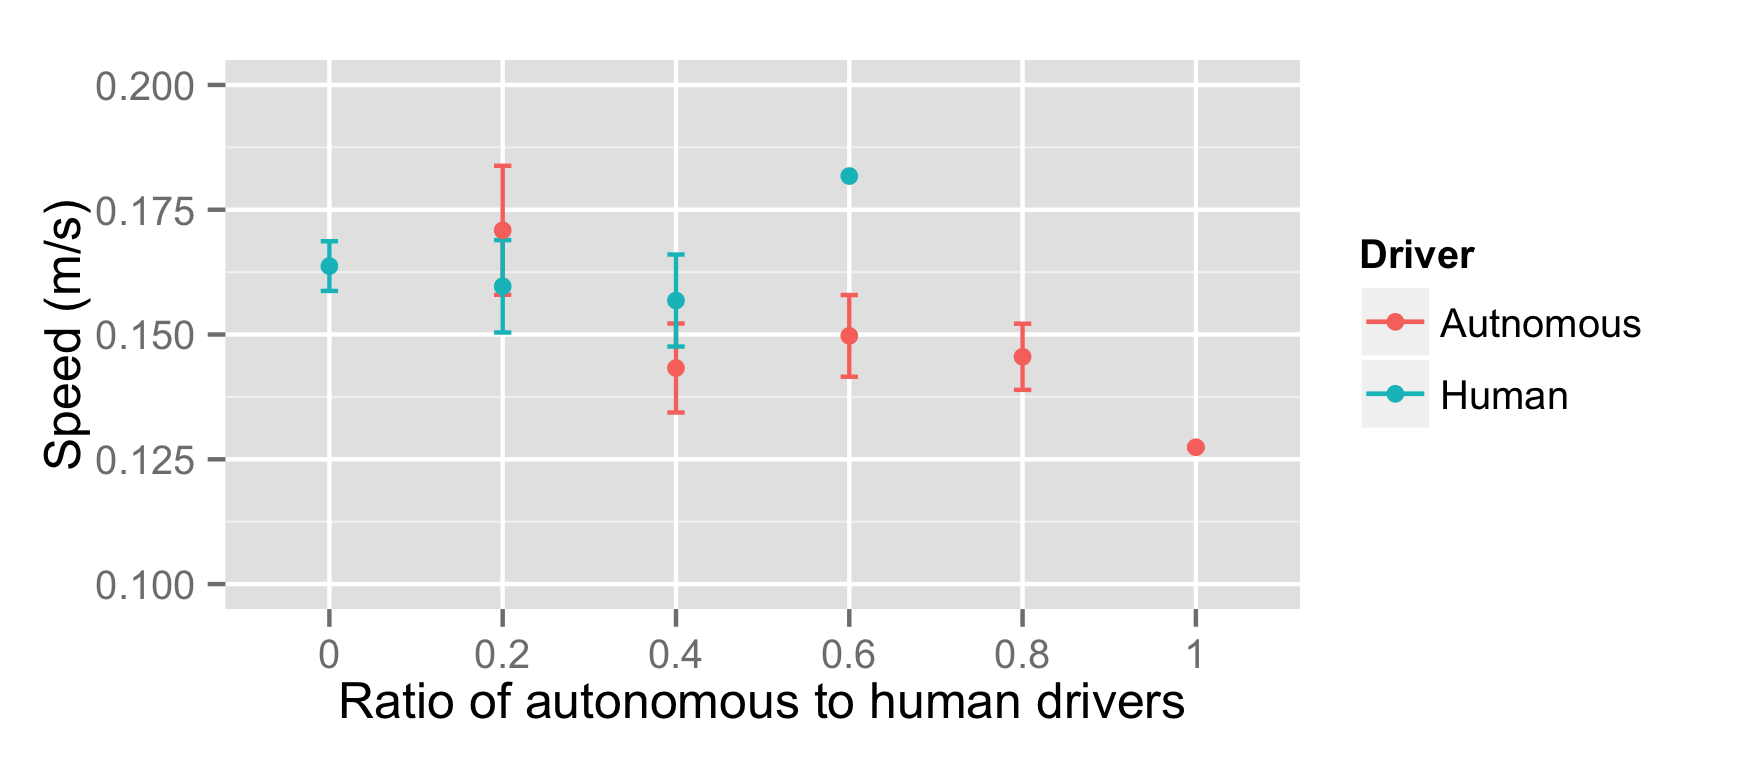
\includegraphics[width=\textwidth]{./img/intersecting_13}
		\caption{The route from node $S_2$ to node $S_3$ and from $S_3$ to node $S_1$.}
		\label{fig:results:intersecting:13}
	\end{subfigure}	
	\begin{subfigure}{\textwidth}
		\centering
		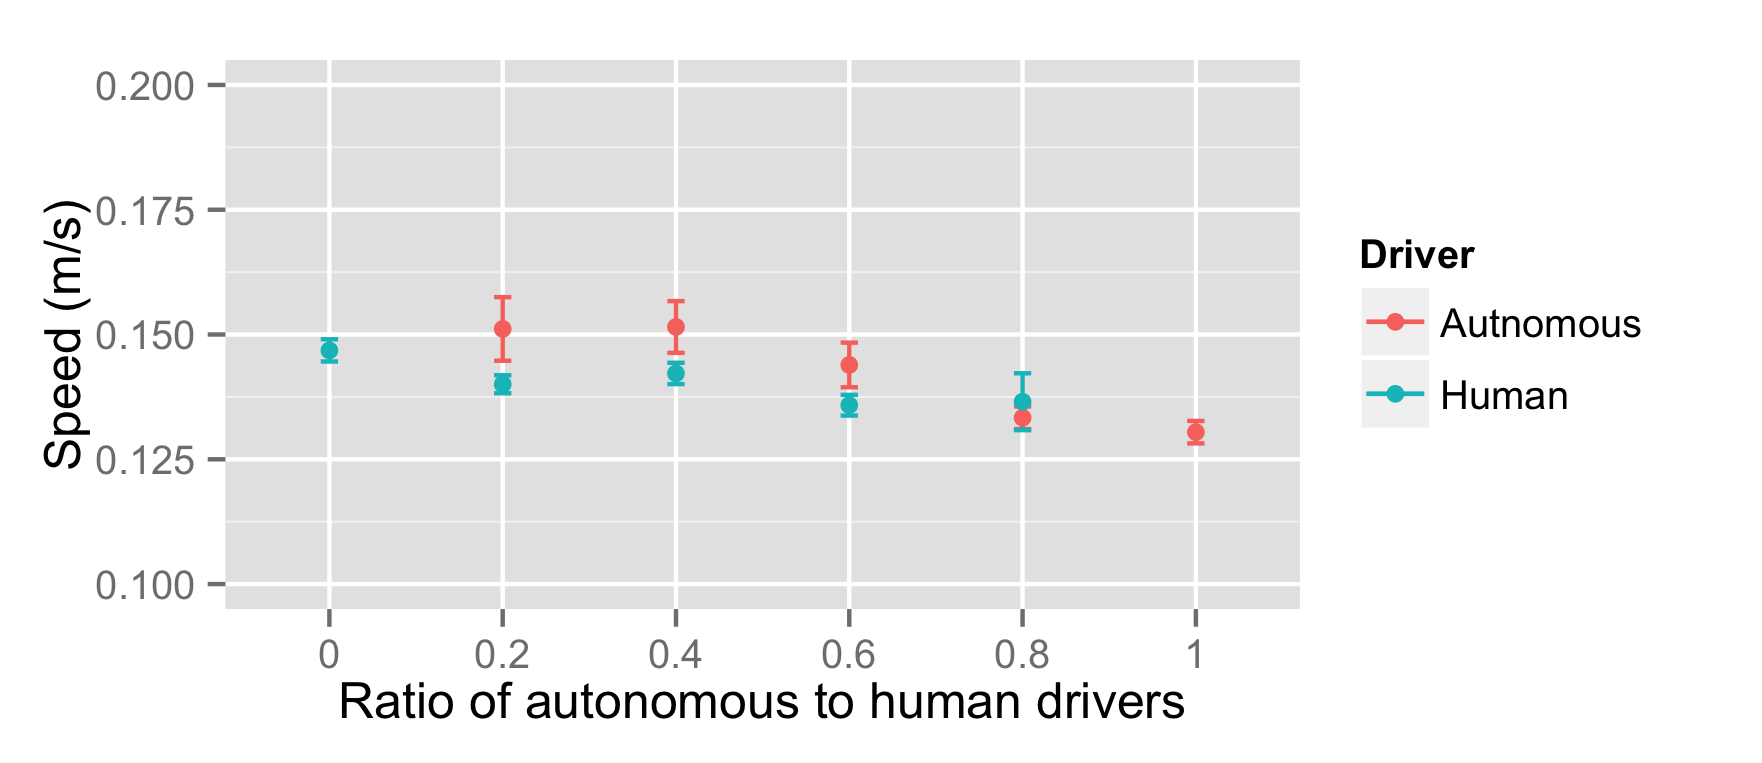
\includegraphics[width=\textwidth]{./img/intersecting}
		\caption{The route of all routes.}
		\label{fig:results:intersecting:all}
	\end{subfigure}		
	\caption{Results of the `intersecting' graph presented in \cref{fig:method:experiment:intersection}. Each figure presents the mean average speed over different iterations as a function of the autonomous to human ratio for a different set of routes. \ref{fig:results:intersecting:03} shows the mean average speed for the routes containing a curve, \ref{fig:results:intersecting:13} for the straight routes, and \ref{fig:results:intersecting:all} shows the mean average speed for all routes.}
	\label{fig:results:intersecting}
\end{figure}

\subsection{Interpretation of Findings}
\label{sub:results:interpretation}
\jelmer{Blaat over plaatjes en tabel}
\jelmer{Prisoners Dillema}
